I dette prosjektet har vi vist at satelittenes posisjon har ekstremt mye å si for hvor nøyaktig lokasjonen blir. I oppgave 4 og 5 har vi regnet på kondisjonstallene til likningen ved forskjellige tidsfeil. Av task 4 ser vi at så lenge vi har nogenlunde spredte satelitter vil ikke forskjellige faktorkombinasjoner av tidsfeil føre til noen nevneverdig økning i kondisjonstall og posisjonsfeil - og dette er faktum i virkeligheten. Til enhver tid finnes det 24 satelitter som kretser rundt jorden. Uansett hvor du befinner deg på jorda, uansett tidspunkt, har du alltid mellom 5 og 8 satelitter i direkte synslinje. Dette gjør at de 4 satelittene som kreves for å fastsette en posisjon nesten alltid vil være spredt, som igjen gjør at GPS kan fastsette posisjonen din med liten feilmargin. Har vi flere satelitter innen rekkevidde, blir posisjonen ytterligere nøyaktig. Har vi derimot satelitter som befinner seg meget nært hverandre, blir den kalkulerte posisjonen katastrofalt feil, opptil flere tusen kilometer, noe som er forkastelig. Grunnen til dette er vist i figur \ref{fig:bunchedsat}. Vi ser at det mulige området posisjonen kan befinne seg innenfor blir vesentlig større med tette satelittposisjoner. Tidsfeilen har altså mer å si for det mulige posisjonsområdet gitt av tettere satelittposisjoner.

\begin{figure}[htbp]
	\centering
	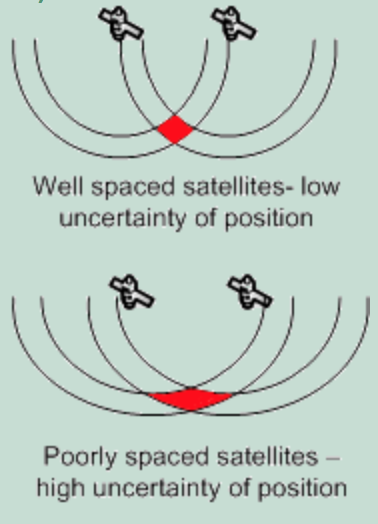
\includegraphics[width=0.4\textwidth]{sections/Conclusion/bunchedsat.png}
	\caption{Klumpede og spredte satelitter}
	\label{fig:bunchedsat}
\end{figure}

Kondisjonstallene og de maksimale posisjonsfeilene regnet i oppgave 4 og 5 er avhengige av satelittposisjonene, så derfor kan ikke disse betraktes som de største mulige verdiene for disse egenskapene. Derfor er egentlig disse tallene lave grenser for kondisjonstallet til GPS-problemet. Av forsøkene og utregningene gjort i oppgave 4 og 5 ser vi at kondisjonstallet vokser utover forsvarlige grenser når satelittene klumpes opp. 

\vspace{5mm}

Måten GPS kalkulerer posisjonen til brukeren er at man vet avstanden fra 3 forskjellige satelitter. Disse 3 avstandene møtes bare i 2 punkter, hvorav ett av disse lett kan utelukkes på grunn av at det ligger utenfor jordas overflate. Dette gjøres ved at hver satelitt sender sin tid til mottakeren, og mottakeren finner hvor langt unna denne satelitten er med å regne tidsforskjellen fra satelittens tid til mottakerens tid, og ganger dette med lyshastigheten. I teorien trenger vi da bare 3 satelitter for å fastsette en posisjon, men på grunn av at mottakerens klokke er relativt unøyaktig i forhold til satelitten, kan dette føre til at posisjonen blir feil med flere kilometer. Derfor trenger vi 4 satelitter for å fastsette den virkelige tiden d, og får derav 4 likninger med 4 ukjente. Her er det verdt å merke seg at hvis vi kunne målt tiden hos mottakeren 100\% nøyaktig, ville den siste satelitten vært unødvendig, og vi kunne funnet posisjonen nøyaktig med 3 satelitter. 

\vspace{5mm}

Andre feilkilder som bidrar til at GPS ikke er 100\% nøyaktig, er at lysfarten ikke er lik fra jordas overflate og opp til satelittene. Dette vil føre til at tiden vi regner med at det tar for signalet å komme frem blir litt unøyaktig, ettersom vi i utregningene har regnet med en konstant lyshastighet c. En annen feilkilde er at vi i denne oppgaven tar det for gitt at signalet fra satelittene går i en rett linje til mottakeren. I virkeligheten har man diverse obstruksjoner som gjør at signalet kan brytes i forskjellige retninger. Dette fører til at mottakeren mottar det samme signalet til forskjellige tider, noe som fører til enda en usikkerhet. Til slutt finnes det i realiteten diverse naturlige og menneskeskapte signaler som vil forstyrre signalet fra satelittene. I figur \ref{fig:errortable} ser vi en oversikt over diverse feilkilder og hvor mye de påvirker posisjonens nøyaktighet \cite{StrangBorre}. I virkeligheten er alle disse problemene enten fjernet helt eller redusert, men i vår oppgave er disse problemene sett bort ifra. Derfor får vi forskjellige resultater enn GPS får i praksis. 

\begin{figure}[h]
	\centering
	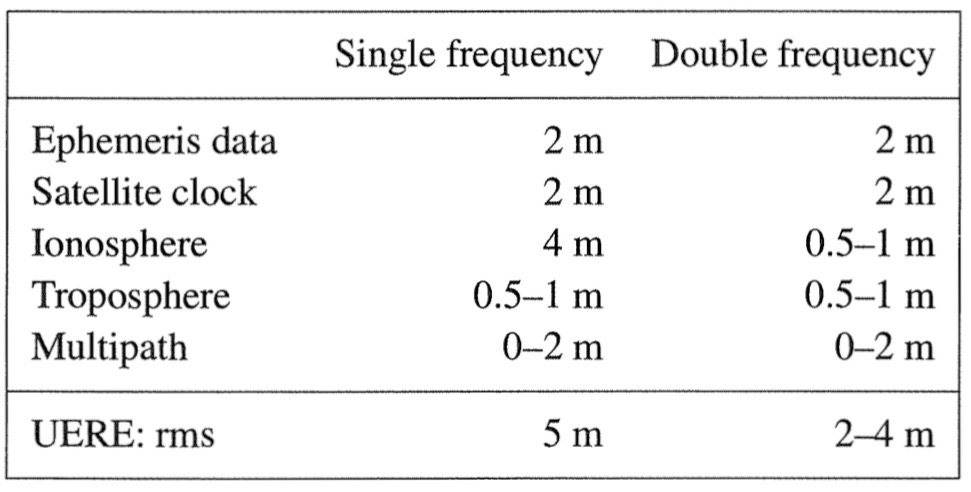
\includegraphics[width=0.60\textwidth]{sections/Conclusion/errortable.jpg}
	\caption{Diverse feilkilder}
	\label{fig:errortable}
\end{figure}